\documentclass[conference]{IEEEtran}
\IEEEoverridecommandlockouts
\usepackage[T1]{fontenc}
\usepackage[utf8]{inputenc}
\usepackage{graphicx}
\usepackage{amsmath,amssymb}
\usepackage{booktabs,tabularx,array}
\usepackage{url}
\usepackage{cite}
\usepackage{microtype}
\newcolumntype{Y}{>{\raggedright\arraybackslash}X}
\renewcommand{\figurename}{Şekil}
\renewcommand{\tablename}{TABLO}
\renewcommand{\refname}{KAYNAKLAR}
\begin{document}

\title{SACI: SIEM-CTI Görünürlük Kanıtlarının Graf Destekli Ölçümü}

\author{\IEEEauthorblockN{İsmet Arslan}
\IEEEauthorblockA{\textit{Bilgisayar Mühendisliği Anabilim Dalı, Lisansüstü Eğitim Enstitüsü}\\
\textit{Karamanoğlu Mehmetbey Üniversitesi}\\
Karaman, Türkiye\\
ORCID: 0009-0005-0274-7989}}

\maketitle

\begin{abstract}
Bir güvenlik bilgi ve olay yönetimi (SIEM) sisteminde çok sayıda alarm bulunması, kritik varlıkların beklenen loglarla izlendiğini veya bu logların çalışan tespitler, MITRE ATT\&CK teknikleri ve tehdit istihbaratıyla izlenebilir biçimde bağlandığını tek başına göstermez. Bu çalışma, sabit ve sürümlenmiş bir kapsam içinde bu ilişkilerin kapanışını ölçen Security Analytics Coverage Index (SACI) yaklaşımını sunmaktadır. SACI; kritik varlık ağırlıklı log kapsamı, etkin kontrol/alarm kapsamı, seçili ATT\&CK teknik kapsamı, CTI entegrasyon iş akışı ve koşum tazeliğini ayrı bileşenler olarak hesaplar. Tiplenmiş kanıt grafı skorun dayandığı varlık--log--kontrol--kural--teknik--IOC zincirini gösterirken, bağımsız bütünlük kapısı bozuk düğüm veya eşleme içeren çıktıları geçersiz sayar. Yöntem altı varlıklı Wazuh--MISP laboratuvarında uygulanmıştır. Kanonik koşumda tanımlı log, kontrol, teknik ve CTI beklentileri kapanmış; seçili telemetri, CTI ve tazelik kayıpları ilgili bileşenlerde beklenen düşüşleri üretmiştir. Sonuçlar SACI'nin güvenlik başarısını değil, tanımlı kapsam içindeki kanıt tamlığını ve bu kanıtın denetlenebilirliğini ölçtüğünü göstermektedir.
\end{abstract}

\begin{IEEEkeywords}
SACI, SIEM, Wazuh, MITRE ATT\&CK, MISP, tespit kapsamı, kanıt grafı, bütünlük doğrulaması
\end{IEEEkeywords}

\begin{center}\textbf{Abstract}\end{center}
{\small A large number of alerts in a security information and event management (SIEM) system does not by itself demonstrate that critical assets are monitored through the expected logs or that those logs are traceably connected to active detections, MITRE ATT\&CK techniques, and threat intelligence. This study presents the Security Analytics Coverage Index (SACI), which measures the closure of these relations within a fixed and versioned scope. SACI separately calculates criticality-weighted log coverage, enabled control and alert coverage, scoped ATT\&CK technique coverage, CTI integration workflow closure, and run-level freshness. A typed evidence graph exposes the asset--log--control--rule--technique--IOC chains behind the scores, while an independent integrity gate rejects outputs with invalid nodes or mappings. The method was applied to a six-asset Wazuh--MISP laboratory. The canonical run closed the declared expectations; selected telemetry, CTI, and freshness losses produced the expected component-level decreases. SACI therefore measures evidence completeness and auditability within a declared scope rather than security effectiveness.\par}
\vspace{2pt}
{\small\textbf{Keywords---}SACI, SIEM, Wazuh, MITRE ATT\&CK, MISP, detection coverage, evidence graph, integrity validation.}

\section{Giriş}
Güvenlik operasyon merkezleri (SOC), farklı işletim sistemleri, ağ cihazları ve güvenlik ürünlerinden gelen olayları SIEM üzerinde bir araya getirir. Buna rağmen logların sisteme ulaşması ile kullanılabilir güvenlik görünürlüğü aynı şey değildir. Bir varlıktan veri geliyor olabilir ancak veri eski olabilir, ilgili tespit kuralı hiç çalışmamış olabilir veya alarmın hangi ATT\&CK tekniği ve tehdit istihbaratı kaydıyla ilişkili olduğu gösterilemeyebilir. SOC çalışmalarında araç, süreç ve insan boyutlarının birlikte değerlendirilmesi gerektiği uzun süredir vurgulanmaktadır \cite{vielberth2020,agyepong2020,sundaramurthy2014}. Açık kaynak SIEM'lere yönelik güncel deneyler de ürünlerin toplama ve performans özelliklerini karşılaştırmakla birlikte, kurumun kendi kapsamındaki kanıt zincirinin ne ölçüde kapandığını ayrı bir problem olarak bırakmaktadır \cite{manzoor2024}.

ATT\&CK tabanlı teknik kapsam bu boşluğu kısmen görünür hâle getirir. DeTT\&CT veri kaynağı kalitesi, görünürlük ve tespit kapsamını puanlamaya yönelik güçlü bir operasyonel araçtır \cite{dettect}. Chamkar ve arkadaşları cihazlardan üretilen olayları ATT\&CK ile eşleyerek SOC use-case kapsamı ve boşluk analizi önermiştir \cite{chamkar2024}. Ancak ATT\&CK etiketi bulunan bir kuralın varlığı tek başına gerçek bir olay üzerinde çalışan bir tespiti kanıtlamaz. Virkud ve arkadaşları da farklı ürünlerdeki ATT\&CK kapsamının düşük önem düzeyli kurallarla şişebildiğini ve aynı tehdit davranışının tutarsız tekniklerle etiketlenebildiğini göstermiştir \cite{virkud2024}. Bu nedenle SACI, ATT\&CK kapsamını bir güvenlik başarısı olarak değil, önceden tanımlı teknik kümesindeki kanıt kapanışı olarak ele alır.

Literatürdeki diğer çizgiler probleme farklı düzeylerden yaklaşır. SOC-CMM insan, süreç, teknoloji ve hizmetler üzerinden SOC olgunluğunu değerlendirir \cite{soccmm}. KRYSTAL gibi bilgi grafı çalışmaları ise audit verisi, tehdit istihbaratı ve tespit yöntemlerini saldırı keşfi ve senaryo yeniden oluşturma için birleştirir \cite{krystal2022}. CTI araştırmaları paylaşım modellerini ve besleme kalitesini inceler \cite{mavroeidis2017,griffioen2020}. Buna karşılık sabit bir kurumsal kapsam içinde varlık, log kaynağı, etkin kontrol, SIEM kuralı, ATT\&CK tekniği ve CTI iş akışını aynı denetlenebilir zincirde tutan; pay ve paydaları yayımlayan ve yapısal olarak bozuk bir çıktı yüksek puan alsa dahi yayını durduran uygulamalı ölçüm protokolleri sınırlıdır.

Bu çalışma bu dar boşluğa odaklanmaktadır. SACI'nin amacı yeni bir risk formülü geliştirmek değil, beş soruya açık yanıt üretmektir: Beklenen loglar geliyor mu? Etkin kontroller gerçekten kanıt veya alarm üretti mi? Kapsam içindeki teknikler geçerli ilişkilere bağlandı mı? CTI entegrasyon zinciri tamamlandı mı? Koşum güncel olay içeriyor mu? Skorun yanında üretilen graf sonuçların kökenini, bütünlük kapısı ise veri paketinin yayımlanabilir olup olmadığını gösterir.

\section{İlgili Çalışmalar ve Araştırma Boşluğu}
\subsection{SOC, SIEM ve Olgunluk Değerlendirmesi}
SOC literatürü güvenlik operasyonlarının yalnız teknoloji seçimine indirgenemeyeceğini; organizasyon, iş akışları, analist yükü ve ölçüm problemlerinin birlikte ele alınması gerektiğini göstermektedir \cite{vielberth2020,agyepong2020,sundaramurthy2014}. SOC-CMM bu yaklaşımı olgunluk değerlendirmesine dönüştürür \cite{soccmm}. Manzoor ve arkadaşları ise Wazuh dâhil açık kaynak SIEM çözümlerini güvenlik özellikleri ve performans bakımından karşılaştırmıştır \cite{manzoor2024}. SACI insan ve süreç olgunluğunu ya da ürün performansını değil, belirli bir SIEM kurulumunda tanımlanmış teknik kanıt beklentilerinin gerçekleşip gerçekleşmediğini ölçer.

\subsection{ATT\&CK Tabanlı Görünürlük ve Tespit Kapsamı}
DeTT\&CT veri kaynağı kalitesi, görünürlük, tespit kapsamı ve tehdit aktörü davranışlarını ATT\&CK üzerinde karşılaştırmak için kullanılan önemli bir pratik tabandır \cite{dettect}. Chamkar ve arkadaşları düşük seviyeli olay ve örüntüleri ATT\&CK tekniklerine bağlayarak use-case kapsamını değerlendirmiştir \cite{chamkar2024}. SACI'nin ayrıldığı nokta, teknik puanını tek başına üretmemesi; teknik kapanışını belirli varlık, log kaynağı, etkin kontrol, kural ve gözlenen alarm ilişkisine bağlamasıdır. Ayrıca veri paketinin yapısal geçerliliği kapsam skorundan bağımsız bir kararla denetlenir. Bu tercih ATT\&CK kapsamının tespit etkinliği olarak yorumlanmasına yönelik ampirik eleştirilerle uyumludur \cite{virkud2024}.

\subsection{CTI ve Kanıt Grafları}
Mavroeidis ve Bromander CTI taksonomileri, paylaşım standartları ve ontolojileri arasındaki parçalanmayı incelemiştir \cite{mavroeidis2017}. Griffioen ve arkadaşları CTI beslemelerinin zamanlılık, duyarlılık, özgünlük ve etki bakımından farklı kalite özellikleri taşıdığını göstermiştir \cite{griffioen2020}. MISP işbirlikçi paylaşım ve gösterge yönetimi için uygulanmış bir platform sunar \cite{wagner2016}. SACI'nin CTIC bileşeni bu kalite boyutlarını ölçmez; Wazuh--MISP hattındaki sorgu, eşleşme, alarm ve ATT\&CK bağlamı adımlarının test kapsamında kapanıp kapanmadığını ölçer.

KRYSTAL, bilgi grafını tehdit tespiti, saldırı grafı ve senaryo yeniden oluşturma için kullanır \cite{krystal2022}. Hogan ve arkadaşları bilgi graflarında şema, kimlik, kalite değerlendirmesi ve yayınlama adımlarının güvenilir veri yönetimi için temel olduğunu vurgular \cite{hogan2021}. SACI grafı ise çıkarım veya saldırı yolu keşfi yapmak yerine skorun hangi ilişki satırlarından üretildiğini göstermeye ve referans bütünlüğünü denetlemeye hizmet eder. Tablo~\ref{tab:comparison} konumlandırmayı özetlemektedir.

\begin{table}[t]
\caption{SACI'nin yakın yaklaşımlarla konumu}
\label{tab:comparison}
\centering
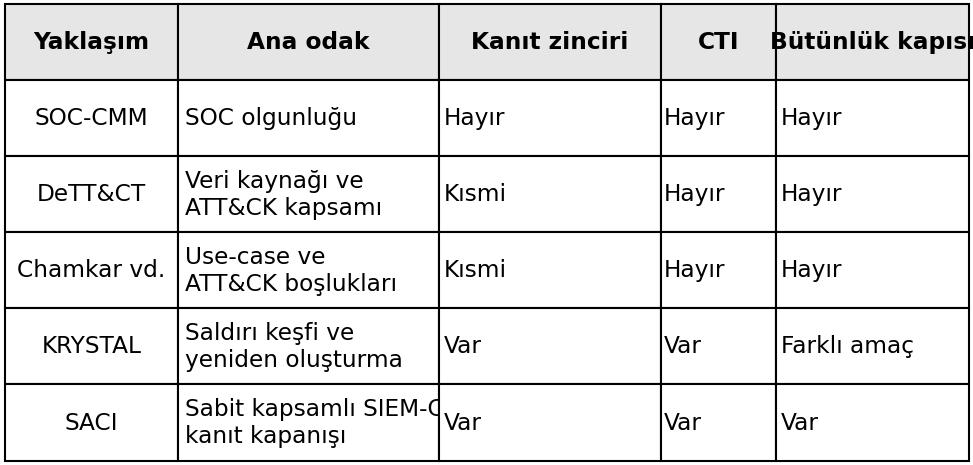
\includegraphics[width=\columnwidth]{figures/comparison.png}
\end{table}

\section{SACI Yöntemi}
\subsection{Uçtan Uca Kanıt Zinciri}
SACI'nin işleyişi iki temsilî yol üzerinden açıklanabilir. İlk yolda DC01 üzerinde hesap veya ağ keşfi davranışı üretilir. Windows Security ya da Sysmon olayı Wazuh tarafından alınır, özel tespit kuralı alarm üretir ve kural kapsam içindeki ATT\&CK tekniğine bağlanır. Böylece aynı gözlem log kapsamına, kontrol kapsamına ve teknik kapsamına kanıt sağlar. İkinci yolda sentetik IOC içeren DNS veya dosya olayı Wazuh--MISP entegrasyonuna iletilir. MISP eşleşmesi zenginleştirme kaydına, Wazuh alarmına ve ATT\&CK bağlamına dönüştürülür. Şekil~\ref{fig:flow} iki yolu ve yayın kararını göstermektedir.

\begin{figure}[t]
\centering
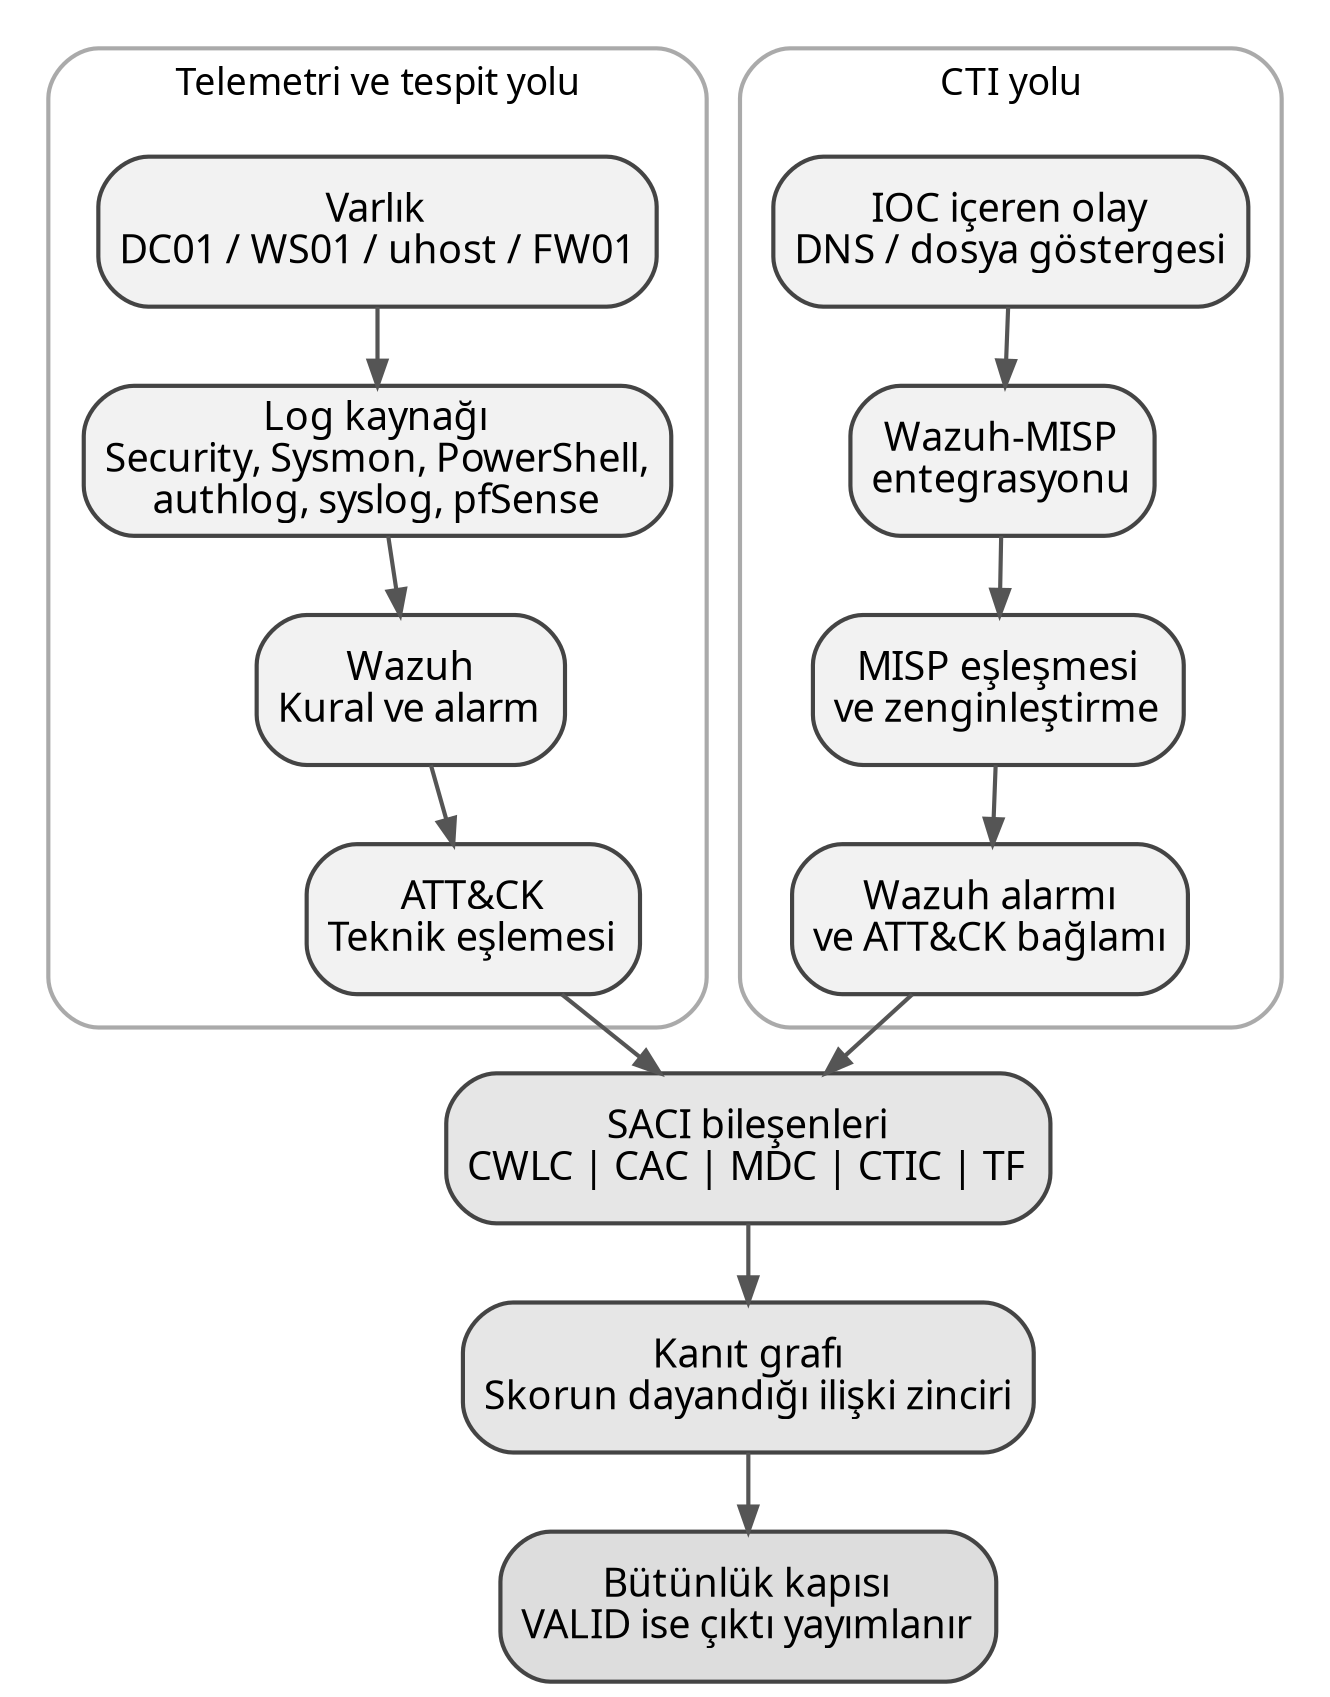
\includegraphics[width=0.98\columnwidth]{figures/flow.png}
\caption{Telemetri/tespit ve CTI kanıt yollarının SACI bileşenleriyle ilişkisi.}
\label{fig:flow}
\end{figure}

\subsection{Kapsam ve Graf Şeması}
Değerlendirme başlamadan önce varlıklar, her varlıktan beklenen log kaynakları, uygulanabilir kontroller, kapsam içindeki ATT\&CK teknikleri ve IOC test kayıtları sürümlü veri dosyalarında tanımlanır. Bu tanım paydadır. Kapsamdan çıkarılan her öğe gerekçe ve sürüm bilgisi taşır; farklı kapsam kimliklerine sahip koşumlar doğrudan karşılaştırılmaz. Etkin olması gereken ancak gözlenmeyen kontrol boşluk olarak kalır. Gerçekten uygulanabilir olmayan veya emekliye ayrılmış kontrol yalnız belgelenmiş politika gerekçesiyle paydadan çıkarılır.

Graf $G=(V,E)$ biçimindedir. $V$; varlık, log kaynağı, kontrol, Wazuh kuralı, ATT\&CK tekniği, IOC, entegrasyon ve metrik düğümlerinden oluşur. $E$ kümesi yönlü ilişkiler içerir. Her ilişki gözlem durumu, kanıt kaynağı ve gerektiğinde benzersiz \texttt{evidence\_id} alanı taşır. Graf bağımsız bir doğrulama veri kümesi değil, skor tablosundaki iddiaların köken görünümüdür.

Teknik kimlikleri Enterprise ATT\&CK matrisinden, CTI nesne semantiği ise STIX 2.1 standardından alınmıştır \cite{mitre_matrix,stix21}. Ölçülerin amaç, kapsam, veri kaynağı, hesaplama yöntemi ve yorum sınırıyla birlikte tanımlanması; NIST sürekli izleme ve bilgi güvenliği ölçüm kılavuzları ile ISO/IEC 27004 ölçüm yaklaşımıyla uyumludur \cite{nist800137,nist80055v1,nist80055v2,iso27004}. Bu operasyonelleştirme, sistem güvenliği metriklerinin açık tanım, kapsam ve yorumlanabilirlik sorunlarını ele alan literatürle de uyumludur \cite{pendleton2016}. Bu kaynaklar SACI ağırlıklarını belirlemez; ağırlıklar deney kapsamında açıkça tanımlanan tasarım parametreleridir.

\subsection{Bileşenler ve Birleşik Skor}
Bileşen skorlarının tümü 0--100 aralığındadır. $A$ varlık kümesini, $L_a$ varlık $a$ için beklenen log kaynaklarını, $c_a$ varlık kritikliğini, $w_{as}$ kaynak ağırlığını ve $o_{as}$ gözlem durumunu gösterir:
\begin{align}
v_a &= \frac{\sum_{s\in L_a} w_{as}o_{as}}{\sum_{s\in L_a} w_{as}}, \\[-2pt]
CWLC &= 100\frac{\sum_{a\in A}c_av_a}{\sum_{a\in A}c_a}. \label{eq:cwlc}
\end{align}
Kontrol/alarm kapsamı (CAC), yalnız uygulanabilir ve etkin kontrol kümesi $C^*$ üzerinde hesaplanır. $u_c$ kontrol ağırlığını, $g_c$ ise geçerli alarm veya kanıt görülme durumunu gösterir:
\begin{equation}
CAC=100\frac{\sum_{c\in C^*}u_cg_c}{\sum_{c\in C^*}u_c}. \label{eq:cac}
\end{equation}
MDC, önceden belirlenen $T_{scope}$ teknik kümesinde en az bir geçerli tespit zinciriyle kapanan tekniklerin oranıdır:
\begin{equation}
MDC=100\frac{\sum_{t\in T_{scope}}z_t}{|T_{scope}|}. \label{eq:mdc}
\end{equation}
CTIC, her sentetik IOC için sorgu adımı $q_i$, MISP eşleşmesi $h_i$, Wazuh alarmı $a_i$ ve ATT\&CK bağlamı $m_i$ olmak üzere dört iş akışı adımını sayar:
\begin{equation}
CTIC=100\frac{\sum_{i\in I}(q_i+h_i+a_i+m_i)}{4|I|}. \label{eq:ctic}
\end{equation}
Mevcut prototipte $q_i$ bağımsız HTTP istek--cevap kaydından değil senaryo beklentisinden başlatılmaktadır. Bu nedenle CTIC, CTI kalitesi veya tam sorgu kökeni değil, yapılandırılmış entegrasyon iş akışının kapanışıdır. TF ise skor zamanı ile koşumdaki en yeni olay arasındaki yaşa göre 100, 80, 50 veya 0 değerini alır; kaynak bazında sağlık ölçümü değildir.

Nihai skor, normalize edilmiş bileşenleri basit toplamsal ağırlıklandırma (Simple Additive Weighting, SAW) mantığıyla birleştirir \cite{triantaphyllou2000}. Bu deneyde ağırlıklar CWLC=0,30, CAC=0,25, MDC=0,20, CTIC=0,15 ve TF=0,10 olarak belirlenmiştir. $M^*$ aktif bileşen kümesi ve $\alpha_j$ bileşen ağırlığıdır:
\begin{equation}
SACI=\frac{\sum_{j\in M^*}\alpha_jM_j}{\sum_{j\in M^*}\alpha_j}. \label{eq:saci}
\end{equation}
Ağırlıklar evrensel veya istatistiksel olarak öğrenilmiş değerler değildir; laboratuvarın önceden açıklanmış öncelikleridir. Zorunlu veri dosyası eksikse, payda sıfırsa ya da aktif bileşen kümesi boşsa sonuç yayımlanmaz.

\subsection{Bütünlük Kapısı ve Neden Kodları}
Skor hesaplaması ile veri bütünlüğü ayrı sonuçlardır. Doğrulayıcı düğüm kimliği benzersizliğini, zorunlu sütunları, kaynak ve hedef uçların düğüm envanterinde bulunmasını, doğrudan ATT\&CK eşlemelerinin tutarlılığını, paralel ilişkilerde \texttt{evidence\_id} benzersizliğini ve CSV--CYJS eşleşmesini denetler. Bu kontrol yaklaşımı, bilgi graflarında şema, kimlik ve kalite doğrulamasını yayınlama sürecinin ayrı bir parçası olarak ele alan genel ilkeleri uygulama grafına uyarlamaktadır \cite{hogan2021}. Zorunlu bir kural ihlal edildiğinde çıktı INVALID veya INCOMPLETE olur; yayın kapısı açılmaz. Kapanmayan bileşenler neden kodlarıyla raporlanır.

\section{Deney Ortamı ve Uygulama}
\subsection{Laboratuvar Topolojisi}
Kontrollü laboratuvar altı mantıksal varlıktan oluşmaktadır. WSIEM merkezi Wazuh toplama ve kural değerlendirme katmanıdır. DC01 ve WS01 Windows olaylarını, uhost Linux günlüklerini, FW01-pfSense ağ olaylarını, CTI01 ise MISP API ve sentetik IOC kayıtlarını sağlar. Windows kanalları ve Linux günlükleri Wazuh toplama yapılandırmalarıyla, pfSense olayları uzak syslog ile aktarılmıştır \cite{wazuhlogs,wazuhapi,sysmon,pfsense}. Şekil~\ref{fig:topology} veri yollarını göstermektedir.

\begin{figure}[t]
\centering
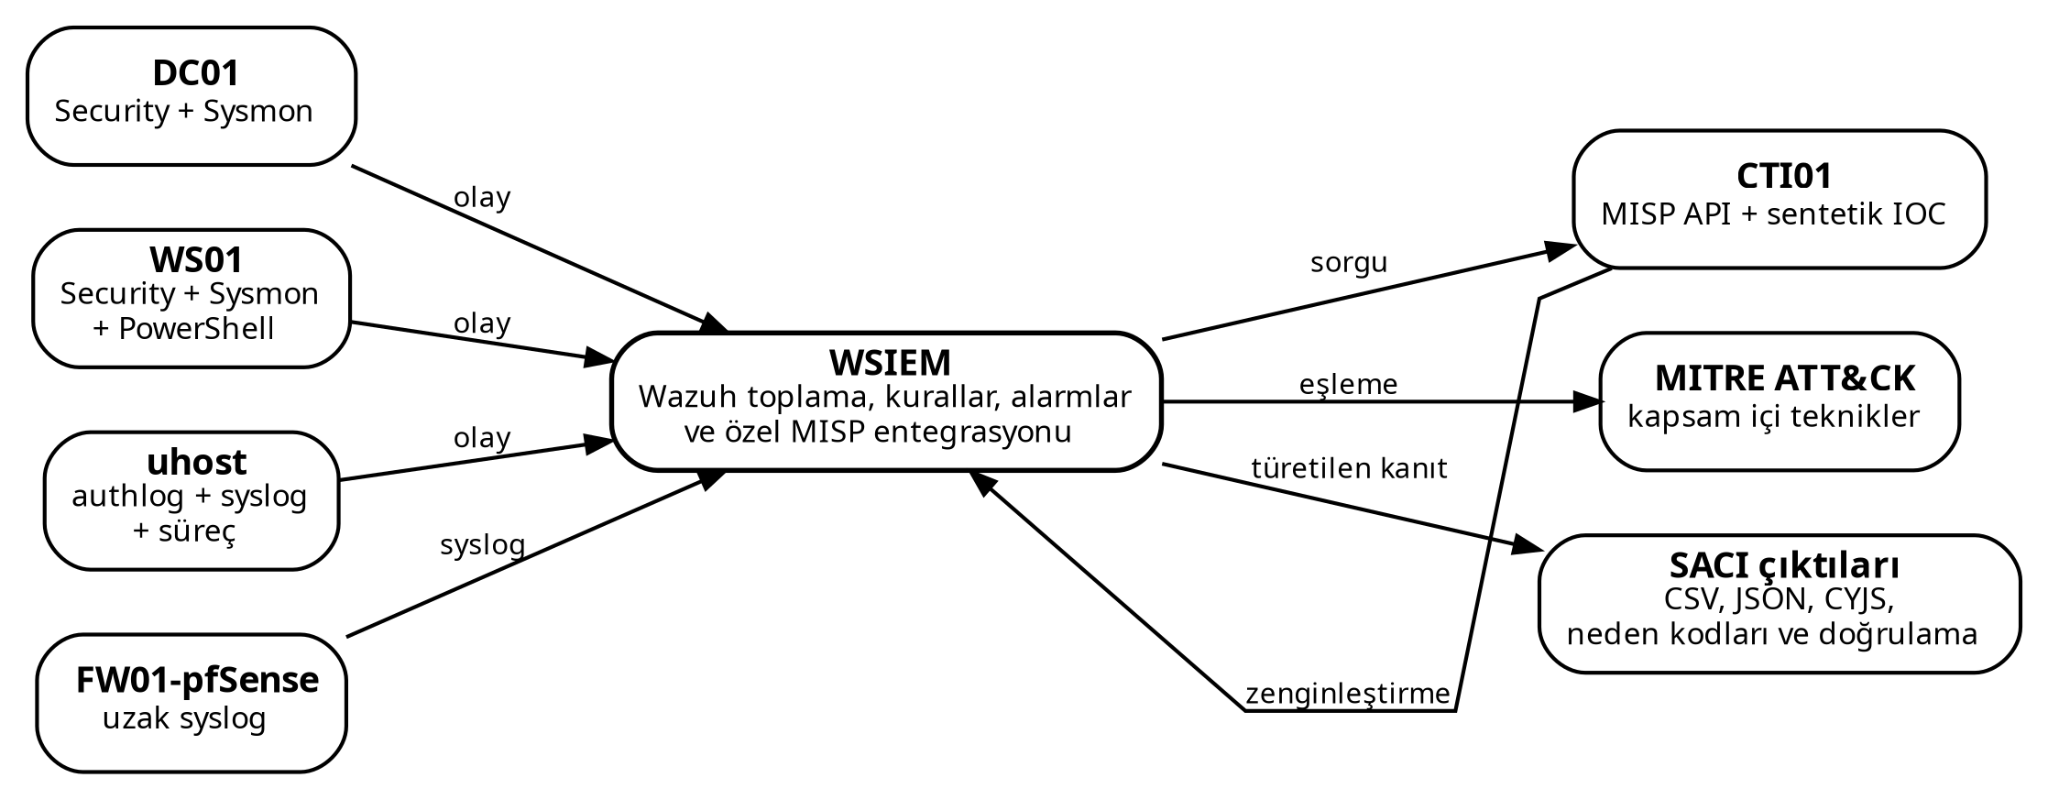
\includegraphics[width=\columnwidth]{figures/topology.png}
\caption{Wazuh--MISP laboratuvarındaki varlıklar ve veri akışları.}
\label{fig:topology}
\end{figure}

\subsection{Kontrollü Davranışlar ve Veri Toplama}
Windows/DC01 yolu Ansible ve WinRM ile çalışan zararsız bir senaryo çalıştırıcısıyla sınanmıştır. Hesap ve etki alanı keşfi, ağ ve paylaşım keşfi, DNS IOC sorgusu ve yerel Python HTTP sunucusundan zararsız dosya aktarımı davranışları üretilmiştir. Her komut senaryo, beklenen ATT\&CK tekniği, kural kimliği ve dönüş koduyla JSONL biçiminde kaydedilmiş; ardından Wazuh alarm dosyasında ilgili kurallar aranmıştır. Linux, pfSense ve CTI yolları için kapsam ve alarm kanıtları kullanılmış, ancak bu yolları baştan kuran eşdeğer saldırı çalıştırıcıları yayımlanmamıştır.

\begin{table}[t]
\caption{Deneyde üretilen temsilî davranışlar}
\centering
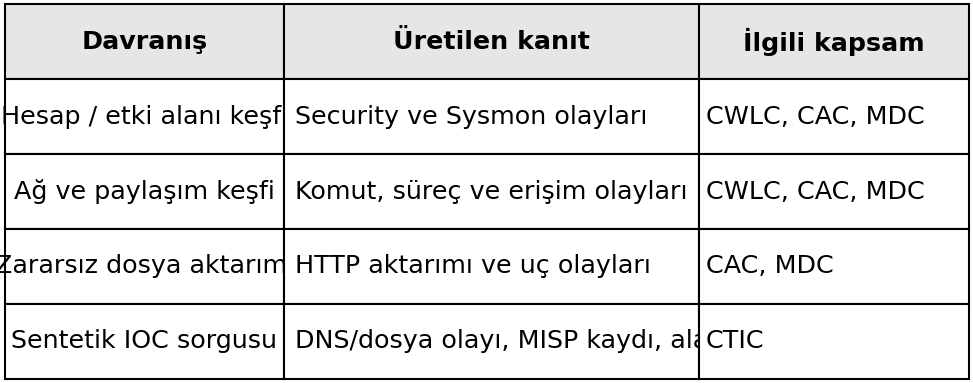
\includegraphics[width=\columnwidth]{figures/behaviors.png}
\end{table}

Skorlayıcı Wazuh alarmlarını, MISP zenginleştirme kayıtlarını, senaryo olaylarını ve pfSense kanıtını normalize eder. Varlık ve log ilişkisi agent adı/kimliği, sağlayıcı, kanal, olay konumu, kural kimliği ve ATT\&CK metaverisiyle kurulur. Aynı normalize tablolardan bileşen skorları ve graf çıktıları türetilir. Araştırma paketi kapsam tablolarını, skor sonuçlarını, graf dosyalarını, neden kodlarını ve doğrulayıcıyı yayımlar \cite{saciartifact}.

\subsection{Değerlendirme Düzeni}
Değerlendirme üç parçadan oluşmaktadır. Birinci parça tüm tanımlı beklentilerin gözlendiği kanonik koşumdur. İkinci parçada kritik ve kritik olmayan telemetri, CTI ve tazelik girdileri kaldırılarak skorun beklenen yönde değişip değişmediği incelenmiştir. Bu senaryolar istatistiksel örneklem değil, formül ve kapsam politikasına yönelik deterministik arıza testleridir. Üçüncü parçada eksik uç, çelişkili eşleme, yinelenen düğüm kimliği ve paralel kanıt çakışması gibi kusurlar enjekte edilerek bütünlük kapısının kararı sınanmıştır.

\section{Sonuçlar}
\subsection{Kanonik Kapsam Sonucu}
Kanonik koşumda altı varlık için tanımlanan 12 varlık--log çiftinin tamamı gözlenmiştir. Emekliye ayrılmış iki legacy kontrol kapsam politikasıyla hariç tutulmuş; kalan 25 etkin kontrolün tamamı geçerli alarm veya kanıt üretmiştir. Kapsam içindeki 13 ATT\&CK tekniği en az bir geçerli tespit zinciriyle kapanmış, iki IOC için dört adımlı CTI iş akışı 8/8 olarak tamamlanmıştır. Koşum tazeliği eşiği de sağlanmıştır.

\begin{table}[t]
\caption{Kanonik SACI sonuçları}
\centering
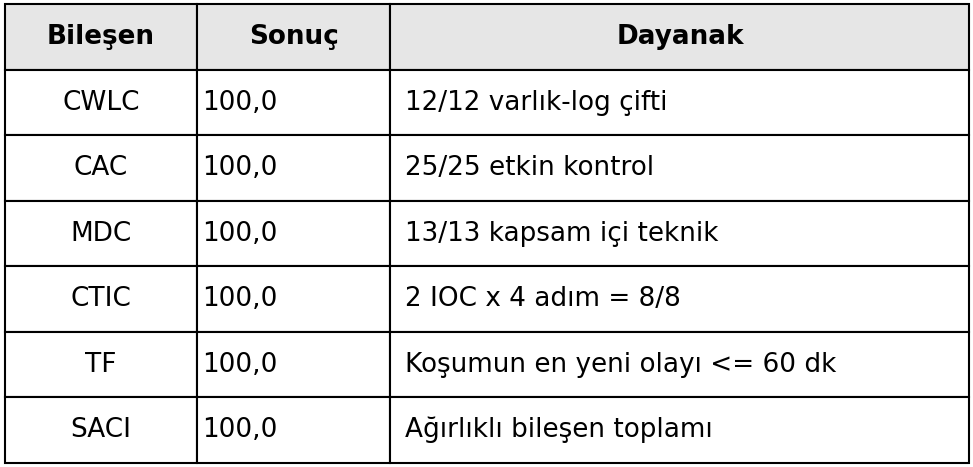
\includegraphics[width=\columnwidth]{figures/results.png}
\end{table}

Sonuç SACI=100'dür. Bu değer laboratuvarın güvenli olduğunu ya da bütün saldırıların algılanacağını göstermez; yalnız tanımlı kapsamın uygulanan gözlem kuralları altında kapandığını gösterir. Birleşik değer bu nedenle her zaman bileşen vektörü, kapsam kimliği ve bütünlük kararıyla birlikte okunmalıdır.

\subsection{Duyarlılık Senaryoları}
Şekil~\ref{fig:sens} seçili arıza senaryolarını göstermektedir. Kritik DC01 Sysmon kaybı skoru 78,53'e düşürmüş, kritik olmayan WS01 kaybı 92,52 üretmiştir. CTI iş akışındaki kayıp 92,50, koşum tazeliğinin gerilemesi ise 95,00 sonucunu vermiştir. Bu sonuçlar kritik varlık ağırlığının ve bileşen ağırlıklarının hesaplamaya beklendiği gibi yansıdığını gösterir; gerçek tespit olasılığı veya nedensel etki büyüklüğü göstermez.

\begin{figure}[t]
\centering
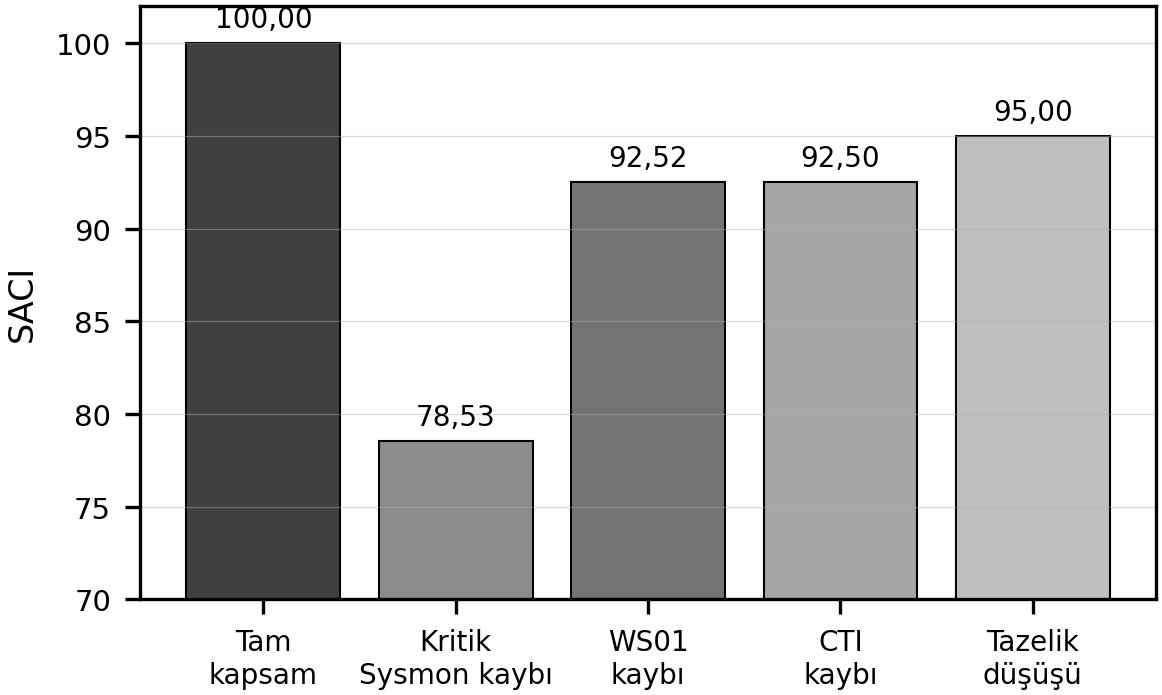
\includegraphics[width=\columnwidth]{figures/sensitivity.png}
\caption{Seçili kanıt kayıplarında SACI değerinin değişimi.}
\label{fig:sens}
\end{figure}

\subsection{Bütünlük Kapısı}
Bütünlük denetimi skor ile graf geçerliliğinin neden ayrı tutulduğunu göstermiştir. Ön yayın paketinde SACI=100 ve bütün ilişki satırları \texttt{observed=1} olmasına karşın iki ilişki ucu düğüm envanterinde yoktu ve bir kuralın doğrudan ATT\&CK eşlemesi CTI bağlamıyla karışmıştı. Bu paket INVALID olarak değerlendirilmiştir. Eksik düğümler eklenmiş, doğrudan eşleme ile bağlamsal ilişki ayrılmış ve paralel kanıtlar benzersiz \texttt{evidence\_id} değerleriyle tanımlanmıştır. Düzeltilen kanonik graf 99 düğüm, 171 ilişki satırı ve sıfır etkin bütünlük bulgusuyla VALID durumuna geçmiştir.

\begin{table}[t]
\caption{Temsilî bütünlük kuralları}
\centering
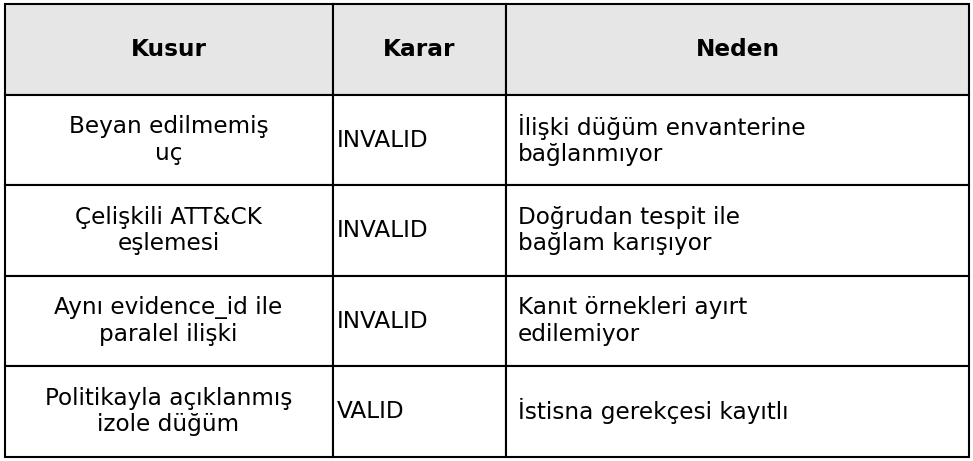
\includegraphics[width=\columnwidth]{figures/integrity.png}
\end{table}

Dokuz kontrollü kusur vakasının her biri beklenen VALID, INVALID veya INCOMPLETE sınıfını üretmiştir. Bu test, bütünlük kapısının yalnız ilk bulunan hataya özel bir düzeltme olmadığını; farklı referans ve şema bozulmalarını ayırabildiğini göstermektedir.

\section{Tartışma}
\subsection{Mevcut Yaklaşımlara Eklenen Değer}
SACI'nin yeniliği ATT\&CK tekniği saymak veya siber güvenlik verisini ilk kez grafa dönüştürmek değildir. DeTT\&CT görünürlük ve tespit kapsamı için daha olgun bir operasyonel taban, Chamkar ve arkadaşlarının yöntemi ise use-case boşluk analizi için doğrudan bir akademik karşılaştırma sunar \cite{dettect,chamkar2024}. SACI'nin katkısı bu kapsama varlık düzeyindeki beklenen log çiftlerini, Wazuh kontrol ve kural gözlemlerini, CTI entegrasyon adımlarını ve fail-closed bütünlük kararını eklemektir. Böylece \texttt{covered=1} değeri yalnız teknik etiketine değil, denetlenebilir ilişki zincirine dayanır.

Graf katmanı da saldırı keşfi yapan KRYSTAL gibi sistemlerle aynı amaçta değildir \cite{krystal2022}. SACI grafı skorun nedenini takip etmeyi ve veri paketi içindeki tutarsızlıkları bulmayı sağlar. Yöntemin uygun kullanım alanları yeni log kaynağı devreye alma kontrolü, sabit kapsamlı görünürlük zaman serisi, denetim öncesi kanıt tamlığı incelemesi ve laboratuvar senaryolarının kapanış kontrolüdür. Farklı kurum veya ürünleri tek SACI değeriyle sıralamak, kapsam ve ağırlıklar kalibre edilmeden savunulamaz.

\subsection{Geçerlik Sınırları}
İlk sınırlama kapsamın önceden tanımlanmasıdır. SACI envanterde bulunmayan varlığı veya seçilmemiş tekniği kendiliğinden keşfetmez. Kapsam daraltılırsa skor yükselebileceği için varlık, kontrol ve teknik paydaları kurumsal envanter veya tehdit modeliyle doğrulanmalı; her çıkarma sürümlenmiş gerekçeyle kaydedilmelidir.

İkinci sınırlama TF ve CTIC bileşenleridir. TF bütün kaynakların en yeni tek olayını kullandığından taze bir kaynak eski akışları maskeleyebilir. Üretim sürümünde tazelik her varlık--log çifti için ayrı hesaplanmalıdır. CTIC içindeki lookup adımı bağımsız istek--cevap kaydına dayanmadığı için sonuç CTI besleme kalitesi veya tam sorgu kökeni olarak yorumlanmamalıdır. Griffioen ve arkadaşlarının ölçtüğü CTI kalite boyutları bu çalışmanın dışında kalmaktadır \cite{griffioen2020}.

Üçüncü sınırlama dış geçerliktir. Deney tek bir altı varlıklı Wazuh--MISP laboratuvarı, iki sentetik IOC ve 13 seçili teknikle yapılmıştır. Duyarlılık senaryoları kodun tanımlı girdilere tepki verdiğini gösterir; yanlış pozitif/negatif oranı, MTTD veya gerçek saldırı tespit başarısı hakkında sonuç üretmez. Bu sorular için farklı SIEM ürünlerinde, gerçek olay kimlikleri ve tekrarlı saha koşumlarıyla ek doğrulama gereklidir.

\subsection{Yeniden Üretilebilirlik}
Yayımlanan paket pay ve paydaların yeniden hesaplanmasına, grafın incelenmesine ve bütünlük kurallarının çalıştırılmasına olanak verir \cite{saciartifact}. Güvenlik araştırmalarında deney adımlarının, veri kaynaklarının ve artefaktların açıkça belgelenmesi ihtiyatlı araştırma uygulaması olarak önerilmektedir \cite{rossow2012}. Aynı girdiler ve analiz adımlarıyla sonuçların yeniden hesaplanması ile bağımsız bir ortamda deneyin yeniden kurulması farklı güvence düzeyleridir \cite{nasem2019}. Buna karşılık özgün ürün sürümleri, tüm Sysmon ve Wazuh yapılandırmaları, kimlik bilgileri ve ham canlı log anlık görüntüsü eksiksiz olarak korunmamıştır. Bu nedenle çalışma sonuç ve artefakt denetimini destekler; özgün laboratuvarın tam dijital ikizini sağlamaz.

\section{Sonuç}
Bu çalışmada SIEM görünürlüğünü varlık, log kaynağı, etkin kontrol, Wazuh kuralı, ATT\&CK tekniği ve CTI iş akışı arasındaki gözlenen ilişkiler üzerinden ölçen SACI sunulmuştur. Altı varlıklı laboratuvarda kanonik kapsam kapanmış, seçili telemetri ve CTI kayıpları ilgili bileşenleri düşürmüş, bütünlük kapısı ise sayısal sonuç tam görünse dahi yapısal olarak bozuk çıktıları engellemiştir.

SACI'nin temel çıktısı tek bir 0--100 değeri değildir. Bileşen vektörü, kapsam sürümü, kanıt grafı, neden kodları ve VALID/INVALID kararı birlikte değerlendirilmelidir. Gelecek çalışma kaynak bazlı tazelik, gerçek CTI istek--cevap kökeni, kapsam dışı varlık keşfi ve farklı SIEM ortamlarında tekrarlı saha doğrulamasına odaklanacaktır.

\section*{Veri ve Araştırma Paketi}
Kapsam ve skor tabloları, düğüm/ilişki dosyaları, neden kodları, bütünlük politikası, doğrulayıcılar ve senaryo serisi SACI Final Evidence Portal üzerinden yayımlanmıştır \cite{saciartifact}.

\IEEEtriggeratref{20}
\bibliographystyle{IEEEtran}
\bibliography{SACI_IDAP26_References}
\end{document}
